\documentclass[8pt]{beamer}
\usefonttheme[onlymath]{serif}


\setbeamertemplate{frametitle}{%
  \vskip1ex
  \usebeamerfont{frametitle}%
  \insertsubsectionhead\par        %  ← 원하는 대로 변경 가능
  \vskip1ex
  \hrule                             % 밑줄(선택)
}

% 테마 선택 (선택 사항)
% \usetheme{Madrid} % 기본 테마, 다른 테마 사용 가능
% \font{serif}
\usepackage{amsfonts}
\usepackage{amssymb}
\usepackage[T1]{fontenc} % To use combination of textbf, textit


% \setcounter{MaxMatrixCols}{20}

% (필요한 패키지들)
% \usepackage{amsthm}
\setbeamertemplate{theorems}[numbered]  % 정리, 정의 등에 번호를 달아줌

% \theoremstyle{plain} % insert bellow all blocks you want in italic
% \newtheorem{theorem}{Theorem}[section] % to number according to section
% 
% \theoremstyle{definition} % insert bellow all blocks you want in normal text
% \newtheorem{definition}{Definition}[section] % to number according to section
% \newtheorem*{idea}{Proof idea} % no numbered block
\usepackage{tcolorbox}

% 필요할 경우 패키지 추가
\usepackage{graphicx} % 이미지 삽입을 위한 패키지
\usepackage{amsmath}   % 수식 사용
\usepackage{hyperref}  % 하이퍼링크 추가
\usepackage{cleveref}
\usepackage{multicol}  % 여러 열 나누기
\usepackage{ulem} % 취소선 및줄 나누기

\usepackage{mathtools}



\newcommand{\mrm}[1]{\mathrm{#1}}
\newcommand{\mbb}[1]{\mathbb{#1}}
\newcommand{\mb}[1]{\mathbf{#1}}
\newcommand{\mc}[1]{\mathcal{#1}}
\newcommand{\tb}[1]{\textbf{#1}}
\newcommand{\ti}[1]{\textit{#1}}
\newcommand{\mypois}[1]{\operatorname{Pois}(#1)}

\newcommand{\mybin}[2]{\operatorname{Bin}\!\left(#1,#2\right)}
\newcommand{\mytoinf}[1]{#1 \rightarrow \infty}
\newcommand{\myexp}[1]{\exp{\left(#1\right)}}
\newcommand{\myunif}[2]{\operatorname{Unif}\!\left(#1, #2\right)}
\newcommand{\mygeom}[1]{\operatorname{Geom}\!\left(#1\right)}
\newcommand{\myexpo}[1]{\operatorname{Expo}\!\left(#1\right)}
\DeclarePairedDelimiter\floor{\left\lfloor}{\right\rfloor}


% 발표 제목, 저자, 날짜 설정
\title{Probability}
\author{Gwanwoo Choi}
% \date{}

\begin{document}
% 표지 슬라이드
\begin{frame}
    \titlepage
\end{frame}

% % 목차 슬라이드
% \begin{frame}
%     \frametitle{Table of Contents}
%     \tableofcontents
% \end{frame}

\subsection{Continuous Random Variable}

\begin{frame}
    \frametitle{Table of Contents}
    \tableofcontents[currentsubsection]
\end{frame}


\begin{frame}{Continuous Random Variable}
    \begin{definition}[Continuous r.v.]
        An r.v. has a continuous distribution if its CDF is differentiable. We also allow there to be endpoints (or finitely many points) where the CDF is continuous but not differentiable, as long as the CDF is differentiable everywhere else. A continuous random variableis a random variable with a continuous distribution.
    \end{definition}

    \begin{definition}[Probability density function]
        For a continuous r.v. $X$ with CDF $F$, the probability density function (PDF) of $X$ is the derivative $f$ of the CDF, given by $f(X) = F^\prime(x)$. The support of $X$, and of its distribution, is the set of all $x$ where $f(x)>0$.
    \end{definition}

    \begin{block}{Proposition 3 (PDF to CDF)}
        Let $X$ be a continuous r.v. with PDF $f$. Then the CDF of $X$ is given by 
        \[F(x) = \int^x_{- \infty} f(t) dt\]
    \end{block}

\end{frame}

\begin{frame}{Continuous Rancom Variable}
    \begin{itemize}
        \item Note that $P(X=x) = 0, \forall x $  in continuous r.v. setting. We can discuss about probability with only integral of PDF.
        \item By the fact $P(X=x)=0, \forall x$, $P(a<X\leq b) = P(a\leq X <b) = P(a< X <b) = P(a \leq X \leq b)$
        \item Because the quantity of PDF $f(x)$ is not a probability, for some values of $x$, it is possible to have $f(x) > 1$.
        \item  Although the height of PDF directly represents the probability, it is closely related to the probability. For small $\epsilon$, 
        \[
            P(3 - \epsilon /2 < X \leq 3 + \epsilon/2 ) = \int_{3- \epsilon/2}^{3 + \epsilon/2} f(x) dx \approx f(x) dx
        \]
    \end{itemize}

    \begin{theorem}[Valid PDFs]
        The PDF $f$ of a continuous r.v. must satisfy the following two criteria:
        \begin{itemize}
            \item Nonnegative: $f(x)\leq 0$
            \item Integrates to $1$: $\int_{-\infty}^\infty f(x) dx = 1$
        \end{itemize}
    \end{theorem}
\end{frame}

\begin{frame}{Continuous Random Variable}
    \begin{example}
        \begin{itemize}
            \item Logistic 
            \[
                F(x; \mu, \sigma) = \frac{\myexp{\frac{x-\mu}{\sigma }}}{1 + \myexp{\frac{x-\mu}{\sigma }}}, \quad f(x; \mu, \sigma) = \frac{\myexp{\frac{x-\mu}{\sigma }}}{\sigma \left(1 + \myexp{\frac{x-\mu}{\sigma }}\right)^2}
            \]
            \item Rayleigh 
            \[
            \begin{gathered}
                F(x; \mu, \sigma) = 1  - \myexp{- \frac{(x-\mu)^2}{2 \sigma^2}}, x > \mu  \\f(x; \mu, \sigma) = \frac{x-\mu}{\sigma^2} \myexp{-\frac{(x-\mu)^2}{2 \sigma^2}}, x > \mu
            \end{gathered}
            \]
        \end{itemize}
    \end{example}

   

    \begin{definition}[Expectation of a continuous r.v.]
        The expected value (also called the expectation or mean) of a continuous r.v. $X$ with PDF $f$ is 
        \[
        E(X) = \int_{-\infty}^\infty x f(x) dx
        \]
    
    \end{definition}
\end{frame}

\begin{frame}{Continuous Random Variable}
    \begin{theorem}[LOTUS, continuous]
        If $X$ is a continuous r.v. with PDF $f$ and $g$ is a function from $\mathbb{R}$ to $\mathbb{R}$, then
        \[
            E[g(X)] = \int_{-\infty}^\infty g(x)f(x) dx
        \]
    \end{theorem}
\end{frame}

\subsection{Uniform Distribution}

\begin{frame}
    \frametitle{Table of Contents}
    \tableofcontents[currentsubsection]
\end{frame}


\begin{frame}{Continuous Random Variable}
    \begin{definition}[Uniform distribution]
        A continuous r.v. is said to have Uniform distribution on the interval $(a,b)$ if its PDF is
        \[
        f(x) = \begin{cases}
            \frac{1}{b-a}\quad \text{if } a<x<b, \\ 0 \quad \text{otherwise},
        \end{cases}
        \]
        This is denoted by $U \sim \myunif{a}{b} $
    \end{definition}

    PDF of uniform distribution $F(x)$ is defined as
    \[
        F(x) = \begin{cases}
            0 \quad \text{if } x\leq a,
            \\ \frac{x-a}{b-a} \quad \text{if } a < x <b,
            \\ 1 \quad \text{if } x \geq b,
        \end{cases}
    \]
\end{frame}

\begin{frame}{Continuous Random Variable}
    Expectation of uniform distribution $U \sim \myunif{a}{b}$ is simply calculated by 
    \[
    E[U] = \int_a^b \frac{x}{b-a} dx = \frac{1}{b-a} \frac{(b-a)^2}{2} = \frac{a+b}{2}
    \]

    $E[U^2]$ is calculated by using the continuous version of LOTUS
    \[
    E[U] = \int_a^b \frac{x^2}{b-a} dx = \frac{1}{b-a} \frac{1}{3}(b^3-a^3) = \frac{b^2 + ab + a^2}{3}
    \]

    By $Var[U] = E[U^2] - E[U]^2$,
    \[
        E[U] = \frac{(a-b)^2}{12}
    \]

\end{frame}

\begin{frame}{Continuous Random Variable}

    \begin{definition}[Location-scale transformation]
        Let $X$ be a random variable and $Y = \sigma X + \mu$, where $\mu$ and $\sigma$ are constants with $\sigma >0$. Then we say that $Y$ has been obtained as a \textit{Location-scale transformation} of $X$. Here $\mu$ controls how the location is changed and $\sigma$ controls how the scale is changed.
    \end{definition}

    \begin{example}
        In a location-scale trainsformation, starting with $X\sim \myunif{a}{b}$ and transforming it to $Y = cX + d$ where $c$ and $d$ are constants with $c >0$, $Y$ is a linear function of $X$ and Uniformity is preserved: $Y \sim \myunif{ca+d}{cb+d}$.  But if $Y$ is defined as a \textit{nonlinear} transformation of $X$, then $Y$ will \textit{not} be Uniform in general. For example, for $X \sim Unif(a,b)$ with $0 \leq a <b$, the transformed r.v. $Y=X^2$ has support $(a^2,b^2)$ but is \textit{not} Uniform on that interval.
    \end{example}

\end{frame}

\begin{frame}{Continuous Random variable}
    Let $U \sim \myunif{0}{1}$. Then 
    \[
    \begin{gathered}
        E[U] = \int_0^1 x dx = \frac{1}{2} \\
        E[U^2] = \int_0^1 x^2 dx = \frac{1}{3} \\
        Var[U] = E[U^2] - E[U]^2 = \frac{1}{3} - \frac{1}{4} = \frac{1}{12} 
    \end{gathered}
    \]
    
    With another uniform distribution $U^\prime \sim \myunif{a}{b}$, $U$ has relation $U^\prime = (b-a)U +a$.
    Then by locaion-scale transformation,
    \[
    \begin{gathered}
        E[U^\prime] = E[(b-a)U+a] = a + (b-a)E[U] = \frac{a+b}{2}\\
        Var[U^\prime] = Var[(b-a)U+a] = Var[(b-a)U] = \frac{(b-a)^2}{12}
    \end{gathered}
    \]

    Via location-scale transformation, it is quite easy to obtain $E[U^\prime]$ and $Var[U^\prime]$.

\end{frame}

\begin{frame}{Continuous Random Variable}
    The technique of location-scale transformation will work for any family of distributions such that shifting and scaling an r.v. whose distribution in the family produces another r.v. whose distribution is in the family. 

\bigskip

    This technique does not apply to families of \textbf{discrete distributions} (with a fixed support) since, for example, shifting or scaling $X \sim \mybin{n}{p}$ changes the support and produces an r.v. that is no longer Binomial. 
    \begin{itemize}
        \item  A Binomial r.v. must be able to take on all integer values between $0$ and some upper bound
        \item but $X + 4$ can't take on any value in $\{0, 1, 2, 3\}$ and $2X$ can only take even values, so neither of these r.v.s has a Binomial distribution.
    \end{itemize}
\end{frame}

\begin{frame}{Continuous Random Variable}
    \begin{theorem}[Universality of the Uniform]
        Let $F$ be a CDF which is a continuous function and strictly increasing on the support of the distribution. This ensures that the inverse function $F^{-1}: (0,1) \mapsto \mathbb{R}$ exist.($F^{-1}$ is sometimes called as the \textit{quantile function}) We than have the following results
        \begin{itemize}
            \item Let $U \sim \myunif{0}{1}$ and $X = F^{-1}$. Then $X$ is an r.v. with CDF $F$.
            \item Let $X$ be an r.v. with CDF $F$. Then $F(X) \sim \myunif{0}{1}$.
        \end{itemize}
    \end{theorem}

    \textit{Proof.}
    \begin{itemize}
        \item Let $U \sim \myunif{0}{1}$ and $X = F^{-1}$. For all real $x$,
         \[P(X \leq x) = P(F^{-1}(U)\leq x) = P(U \leq F(x)) = \int_0^{F(x)} 1 du =F(x)\]
        \item Let $X$ have CDF, and find the CDF of $Y = F(X)$. Since $Y$ takes values in $(0,1)$, 
        \begin{itemize}
            \item $P(Y\leq y)$ equals $0$ for $y \leq 0$
            \item $P(Y\leq y)$ equals $1$ for $y \geq 1$
            \item For $y \in (0,1)$, $P(Y \leq y) = P(F(X) \leq y) = P(X \leq F^{-1}(y)) = F(F^{-1}(y)) = y$
        \end{itemize}
        Thus $Y$ has the $\myunif{0}{1}$ CDF.
    \end{itemize}
    \textit{Recall}: PDF of uniform distribution $F(x)$ is defined as
    \[
        F(x) = \begin{cases}
            0 \quad \text{if } x\leq a,
            \\ \frac{x-a}{b-a} \quad \text{if } a < x <b,
            \\ 1 \quad \text{if } x \geq b,
        \end{cases}
    \]

\end{frame}

\begin{frame}{Continuous Random Variable}
    \begin{example}[Universality with Logistic]
        The Logistic CDF is $F = \frac{e^x}{1+e^x}, \forall x \in \mathbb{R}$ and $F^{-1} = \log{\frac{u}{1-u}}, \forall u \in (0,1)$. If we plug $U \sim \myunif{0}{1}$ in $F^{-1}$, then $F^{-1}(U) = \log{\frac{U}{1-U}}$.
        \[\forall x \in \mathbb{R},
        P\left(\log{\frac{U}{1-U}}\leq x\right) = P\left(U \leq \frac{e^x}{1+ e^x} \right)
        \]
        $\therefore \log{\frac{U}{1-U}} \sim$ Logistic. And also, $F(X) = \frac{e^X}{1+e^X} \sim \myunif{0}{1}$ 
    \end{example}
    \begin{figure}
        \centering
        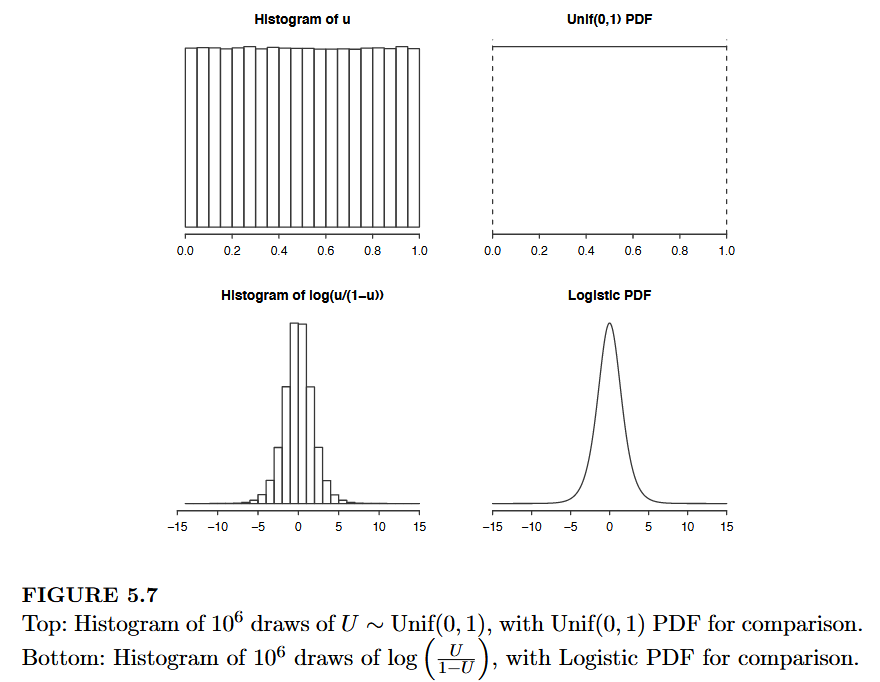
\includegraphics[width=0.45\textwidth]{fig1.png}
    \end{figure}
\end{frame}

\begin{frame}{Continuous Random Variable}
    \begin{example}[Universality with Rayleigh]
        The Rayleigh CDF is $F = 1 - e^{- x^2/2}, \forall x \in \mathbb{R}$ and $F^{-1} = \sqrt{-2 \log{(1-u)}}, \forall u \in (0,1)$.
        $U \sim \myunif{0}{1} \implies \sqrt{-2 \log{(1-U)}} \sim $Layleigh, and $X \sim \text{Rayleigh} \implies F(X)=1-e^{-X^2/2} \sim \myunif{0}{1}$.
    \end{example}
    \begin{figure}
        \centering
        
\includegraphics[width=0.52\textwidth]{fig2.png}
    \end{figure}
\end{frame}

\begin{frame}{Continuous Random Variable}
    Is Universality of the Uniform can be applied to discrete r.v.? Partially, yes.
    For discrete r.v., it's CDF function doesn't have inverse $F^{-1}$ because $F$ of discrete r.v. has jumps and flat regions. We can instead using PMF.

    Suppose we want to use $U \sim \myunif{0}{1}$ to construct a discrete r.v. $X$ with PMF $p_j = P(X=j)$ for $j=0,1,2,\dots,n$.
    Consider the following trick that chop up the interval $(0,1)$ into pieces of lengths $p_0, p_1, \dots, p_n$
    
    \begin{figure}
        \centering
        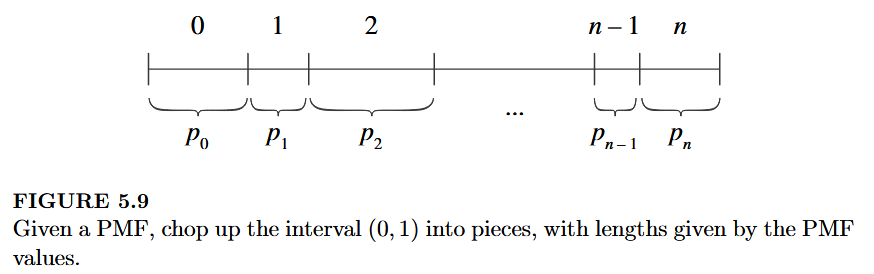
\includegraphics[width=0.6\textwidth]{fig3.png}
    \end{figure}

    The probability $P(X=j)$ is the probabiliy that $U$ falls into the interval of length $p_j$. But for a $\myunif{0}{1}$ r.v., probability is length, so $P(X=j)$ is precisely $p_j$, as desired

\bigskip
    For discrete r.v.,
    \begin{itemize}
        \item Let $U \sim \myunif{0}{1}$ and $X = F^{-1}$. Then $X$ is an r.v. with CDF $F$.
        \item \sout{Let $X$ be an r.v. with CDF $F$. Then $F(X) \sim \myunif{0}{1}$.}
    \end{itemize}


\end{frame}

\begin{frame}{Continuous Random Variable}
    \begin{definition}[Survival function]
        The survival function of an r.v. $X$ with CDF $F$ is the function $G$ given by $G(x) = 1 - F(x) = P(X>x)$.
    \end{definition}
    \begin{theorem}[Expectation by integrating the survival function]
        Let $X$ be a \textbf{nonnegative} r.v. Its expectation can be found by integrating its survival function:
        \[
        E[X] = \int_0^\infty P(X>x)dx
        \]
    \end{theorem}

    Proof. Let $I(x>t)$ be $1$ if $x\geq t$ and $0$ otherwise. Then $\forall x > 0$, $x = \int_0^x dt = \int_0^\infty I(x>t) dt$. So $X = \int_0^\infty I(X>t) dt$. Taking the expectation of both sides and swapping the $E$ with the integral (which can be justified using results from real analysis), we have
    \[E[X] = E\left[\int_0^\infty I(x>t)dt \right] = \int_0^\infty E[I(X>t)]dt  = \int_0^\infty P(X>t)dt\].
\end{frame}

\begin{frame}{Continuous Random Variable}
    \begin{figure}
        \centering
        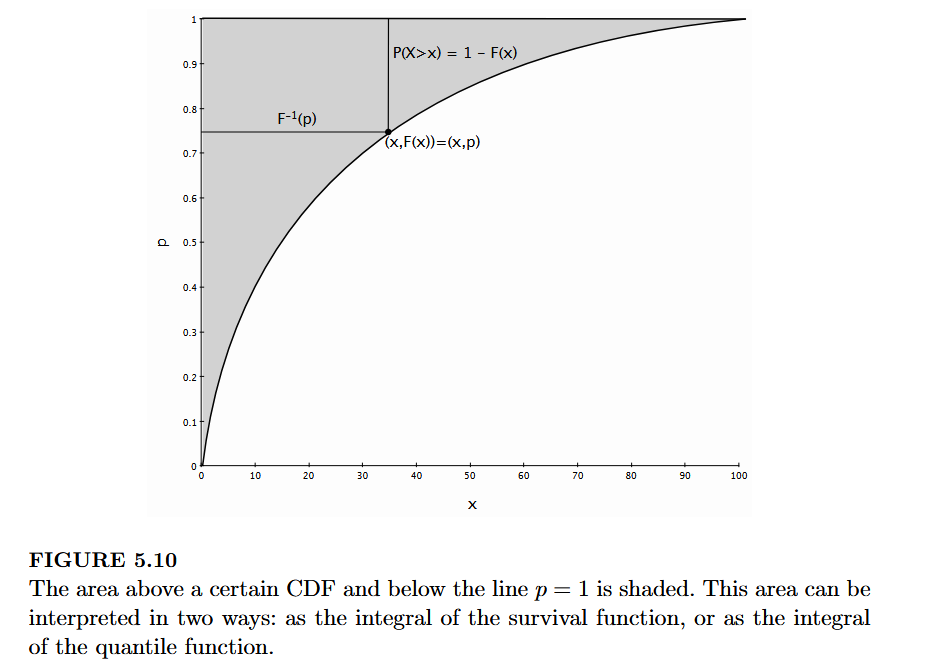
\includegraphics[width=0.63\textwidth]{fig4.png}
    \end{figure}

    For $U \sim \myunif{0}{1}$, \[\int_0^1 F^{-1}(u) du = E_{U}[F^{-1}(U)]= E[X]\]

\end{frame}

\subsection{Normal Distribution}

\begin{frame}
    \frametitle{Table of Contents}
    \tableofcontents[currentsubsection]
\end{frame}

\begin{frame}{Normal Distribution}
    \begin{definition}[Standard Normal distribution]
        A continuous r.v. $Z$ is said to have the \textit{Standard Normal distribution} if its PDF $\varphi$ is given by
        \[\varphi (z) = \frac{1}{\sqrt{2\pi}} e^{-z^2/2}, Z \in \mathbb{R}\]
        We write this as $Z \sim \mathcal{N}(0,1)$
        The Standard Normal CDF $\Phi$ is the accumulated area under the PDF
        \[ \Phi(z) = \int^z_{-\infty} \varphi(t) dt = \int^z_{-\infty}\frac{1}{\sqrt{2\pi}}e^{-t^2/2}dt\]
    \end{definition}
\end{frame}

\begin{frame}{Normal Distribution}
    Check that $\varphi$ satisfies property of PDF, $\int_{-\infty}^\infty \varphi =1$. First, calculate $\int_{-\infty}^\infty e^{-z^2/2}dz$.
    \[
    \begin{gathered}
        \left( \int_{-\infty}^\infty e^{-z^2/2} dz \right)\left( \int_{-\infty}^\infty e^{-z^2/2} dz \right) =  \left( \int_{-\infty}^\infty e^{-x^2/2} dx \right)\left( \int_{-\infty}^\infty e^{-y^2/2} dy \right)\\
        = \int_{-\infty}^\infty \int_{-\infty}^\infty e^{-\frac{x^2 + y^2}{2}} dx dy = \int_{0}^{2\pi} \int_{0}^{\infty} e^{-r^2 /2} r dr d\theta = \int_{0}^{2\pi} \int_0^\infty e^{-u} du d\theta =\int_0^{2\pi} 1 d\theta = 2\pi  \\
        \therefore  \left( \int_{-\infty}^\infty e^{-z^2/2} dz \right) = \sqrt{2\pi}
    \end{gathered}
    \]
    So,
    \[
    \int_{-\infty}^{\infty} \frac{1}{\sqrt{2\pi}}e^{-z^2/2} dz = 1
    \]
    And $\varphi$ is a valid PDF.

\end{frame}

\begin{frame}{Normal Distribution}
    How can we calculate mean and variance of Standard Normal distribution?
    \[E[Z] = \int_{-\infty}^\infty \frac{1}{\sqrt{2\pi}} z e^{-z^2/2} dz = -\int_{\infty}^0 \frac{1}{\sqrt{2\pi}} (-z)e^{-(-z)^2/2} dz + \int_0^\infty \frac{1}{\sqrt{2\pi}}ze^{-z^2/2}dz = 0\]
    Also, variance of $Z$ can be calculated by
    \[
    \begin{gathered}
        Var[Z] = E[Z^2] - E[Z]^2 = E[Z^2]\\
        \begin{aligned}
            E[Z^2] &=  \frac{2}{\sqrt{2\pi}}\int_0^{\infty}z^2 e^{-z^2/2} dz = \frac{2}{\sqrt{2\pi}}\int_0^\infty z\cdot ze^{-z^2/2}dz \\
            &= \frac{2}{\sqrt{2\pi}}\left(\left[z \cdot e^{- z^2 /2} \right]_\infty^0 -\int_0^\infty e^{-z^2/2} dz\right) = \frac{2}{\sqrt{2\pi}}\frac{\sqrt{2\pi}}{2} = 1
        \end{aligned}\\
        \therefore Var[Z] = 1
    \end{gathered}
    \]
\end{frame}

\begin{frame}{Normal Distribution}
    \begin{definition}[Normal Distribution]
        If $Z \sim \mathcal{N}(0,1)$, then $X = \sigma Z + \mu$ is saidto have the \textbf{Normal distribution} with mean $\mu$ and variance $\sigma^2$, for any real $\mu$ and $\sigma^2, \sigma > 0$. We denote this by $X \sim \mathcal{N}(\mu, \sigma^2)$.
    \end{definition}

    \begin{itemize}
        \item \(E[X] = \sigma E[Z]+\mu = \mu\)
        \item \(Var[X] = \sigma^2 Var[Z] = \sigma^2\)
        \item $\frac{X - \mu}{\sigma} \sim \mathcal{N}(0, 1)$
    \end{itemize}

    \begin{theorem}[Normal CDF and PDF]
        Let $X \sim \mathcal{N}(\mu, \sigma^2)$. Then the CDF and PDF of X is 
        \[
        F(x) = \Phi\left(\frac{x-\mu}{\sigma}\right) \qquad f(x) = \varphi\left(\frac{x-\mu}{\sigma}\right)\frac{1}{\sigma}
        \]
    \end{theorem}
    \textit{Proof.} For the CDF, we start from the definition $F(x) = P(X\leq x)$, standardize and use the CDF of the standard Normal:
\[
\begin{gathered}
    F(x) = P(X\leq x) = P\left(\frac{X-\mu}{\sigma}\leq \frac{x-\mu}{\sigma}\right) = \Phi\left(\frac{x-\mu}{\sigma}\right)\\
    f(x) = \frac{1}{\sigma}\varphi\left(\frac{x-\mu}{\sigma}\right) \text{(by chain rule)}
\end{gathered}
\]

\end{frame}

\begin{frame}{Normal Distribution}
    So from $\varphi(z) = \frac{1}{\sqrt{2\pi}} e^{-z^2/2}$ and $f(x) = \frac{1}{\sigma} \varphi\left(\frac{x-\mu}{\sigma}\right)$,
    \[f(x) = \frac{1}{\sqrt{2\pi}\sigma} \exp{\left(- \frac{(x-\mu)^2}{2\sigma^2}\right)}\]

    \begin{itemize}
        \item As we will see later in the book, several important distributions can be obtained through transforming Normal r.v.s in natural ways (squaring or exponentiating). 
        \item Chapter 8 delves into transformations in depth, but meanwhile there is a lot that we can do just using LOTUS and properties of CDFs.
    \end{itemize}
\end{frame}

\begin{frame}{Normal Distribution}
    \begin{example}[Folded Normal]
        Let $Y = \vert Z \vert$ with $Z \sim \mathcal{N}(0,1)$ The distribution of $Y$ is called a \textbf{Folded Normal} with parameters $\mu=0$ and $\sigma^1=1$.

        \begin{enumerate}
            \item[a] Find $E[Y]$
            \item[b] Find $Var[Y]$
            \item[c] Find the CDF and PDF of $Y$ 
        \end{enumerate}

        \textit{Solution(a):} \[
        \begin{aligned}
            E[Y] &= E[\vert Z \vert] = \int_{-\infty}^\infty \frac{1}{\sqrt{2\pi}} \vert z \vert e^{- {\vert z\vert}^2/2} dz = 2 \int_0^\infty \frac{1}{\sqrt{2\pi}}z e^{-z^2 /2}dz \\ &= 2\int_0^\infty \frac{1}{\sqrt{2\pi}} e^{-t} dt
            = 2\left[ \frac{1}{\sqrt{2\pi}} e^{-t} \right]_\infty^0 = \sqrt{\frac{2}{\pi}}
        \end{aligned}
        \]

        \textit{solution(b):} $E[Y^2] = E[Z^2]$ and $E[Z^2] = 1$.
        $\therefore Var[Y^2] = E[Y^2] - E[Y]^2 = 1 - \frac{2}{\pi}$.
        \textit{solution(c):} For $y \leq 0, F_Y(y) = 0$. For $y >0,$
        \[\begin{aligned}
            F_Y(y) &= P(Y \leq y) = P(-y \leq Z  \leq y) = \Phi(y) - (1 - \Phi(y))\ (\text{By symmetricity of } \Phi) \\
            &= 2\Phi(y) -1\
        \end{aligned}
        \]
        By derivative, PDF of $Y$ is $2\varphi(y)$ for $y\geq 0$ and $0$ for $y < 0$. \textit{Note that} although $2\Phi(y) -1$ is not differentiable at $y=0$, $2\Phi(y) -1$ is continuous for $y \in \mathbb{R}$.
    \end{example}
\end{frame}


\subsection{Exponential}

\begin{frame}
    \frametitle{Table of Contents}
    \tableofcontents[currentsubsection]
\end{frame}

\begin{frame}{a}
    \begin{itemize}
        \item The \textbf{Exponential distribution} is the continuous counterpart to the Geometric distribution $\mygeom{\lambda}$.
        \item \textit{Recall.} Geometric random variable counts the number of failures before the first success in a sequence of Bernoulli trials. For $X \sim \mygeom{\lambda}$, $P(X=k) = (1-\lambda)^{k-1}\lambda$, where $\lambda$ is success probability.
        \item We are now waiting for a success in \textit{continuous} time, where success arrive at a rate of $\lambda$ successes per unit of time.
        \item The average number of successes in a time interval of length $t$ is $\lambda t$, though the actual number of successes varies randomly.
    \end{itemize}

    \begin{definition}[Exponential distribution]
        A continuous r.v. $X$ is said to have the \tb{Exponential distribution} with parameter $\lambda$, where $\lambda > 0$, if its PDF is
        \[
        f(x) = \lambda e^{-\lambda x}, x>0
        \] 
        This is denoted by $X \sim \myexpo{\lambda}$.
        The corresponding CDF is 
        \[
        F(x) = 1 - e^{-\lambda x}, x>0
        \]
    \end{definition}

\end{frame}

 \begin{frame}{a}
    \begin{examples}[5.43]
        Suppose that Bernoulli trials are being performed in continuous time; rather than only thinking about first trial, second trial, etc., imagine that the trials take place at points on a timeline. Assume that the trials are at regularly spaced times $0, \Delta t, 2\Delta t, \dots,$ where $\Delta t$ is a small positive number. Let the probability of success of each trial be $\lambda \Delta t$, where $\lambda$ is a positive constant. Let $G$ be the number of failures before the first success (in discrete time), and $T$ be the time of the first success (in continuous time).
        \begin{enumerate}
            \item Find a simple equation relating $G$ to $T$.
            \item Find the CDF of $T$.
            \item Show that as $\Delta t\rightarrow 0$, the CDF of $T$ converges to the $\myexpo{\lambda}$ CDF, evaluating all the CDFs at fixed $t \geq 0$.
        \end{enumerate}
    \end{examples}
    \textit{Solution(1):} $T = \Delta t (G+1)$. ($P(G=k) = (1- \lambda \Delta t)^k \lambda \Delta t$)

    \textit{Solution(2):} \[\begin{gathered}
        P(T \leq t) = P(\Delta t (G+1) \leq t) = P(G \leq \frac{t}{\Delta t} -1) = P(G \leq \left\lfloor \frac{t}{\Delta t} \right\rfloor - 1) \\
        = \sum_{k=0}^{\left\lfloor \frac{t}{\Delta t}\right\rfloor - 1} (1-\lambda \Delta t)^ \lambda \Delta t = \frac{1 - (1 - \lambda \Delta t)^{\left\lfloor\frac{t}{\Delta t} \right\rfloor}}{\lambda \Delta t} \lambda \Delta t = 1 - (1-\lambda \Delta t)^{\left\lfloor \frac{t}{\Delta t}\right\rfloor}
    \end{gathered}
    \]


 
 \end{frame}

 \begin{frame}{a}
    \begin{enumerate}
        \item[3.] Show that as $\Delta t \rightarrow 0$, the CDF of T converges to the $\myexpo{\lambda}$ CDF, evaluating all the CDFs at a fixed $t \geq 0$.
    \end{enumerate}

    \textit{Solution(1):} $T = \Delta t (G+1)$. ($P(G=k) = (1- \lambda \Delta t)^k \lambda \Delta t$)

    \textit{Solution(2):} \[\begin{gathered}
        P(T \leq t) = P(\Delta t (G+1) \leq t) = P(G \leq \frac{t}{\Delta t} -1) = P(G \leq \left\lfloor \frac{t}{\Delta t} \right\rfloor - 1) \\
        = \sum_{k=0}^{\left\lfloor \frac{t}{\Delta t}\right\rfloor - 1} (1-\lambda \Delta t)^ \lambda \Delta t = \frac{1 - (1 - \lambda \Delta t)^{\left\lfloor\frac{t}{\Delta t} \right\rfloor}}{\lambda \Delta t} \lambda \Delta t = 1 - (1-\lambda \Delta t)^{\left\lfloor \frac{t}{\Delta t}\right\rfloor}
    \end{gathered}
    \]

    \textit{Solution(3):}
    \[
    \begin{gathered}
        \lim_{\Delta t \rightarrow 0} F_T(t) = 1 - \lim_{\Delta t \rightarrow 0} (1- \lambda \Delta t)^{\frac{t}{\Delta t}} = 1- \myexp{-\lambda t}
    \end{gathered}
    \]

    This example shows the relationship between Exponential distribution and Gemoetric distribution. With more faster and faster Bernoulli trials and smaller and smaller success probability, We can get Exponential distribution.


 
 \end{frame}

 \begin{frame}{a}
 \begin{example}[location-scale transformation for Exponential distribution]
    Suppose $X \sim \myexpo{1}$. Let r.v. $Y= \frac{X}{\lambda}$. Then $Y \sim \myexpo{\lambda}$.

    Since \[P(Y\leq y) =P(X \leq \lambda y) = 1 - e^{-\lambda y}, \forall y >0
    \]

    Then, we can get mean and variance of $\myexpo{\lambda}$ via $E[\frac{X}{\lambda}] = \frac{1}{\lambda} E[X]$ and $Var [\frac{X}{\lambda}] = \frac{1}{\lambda^2} Var[X]$.

    $E[X] = \int_0^\infty x e^{-x} dx = \left[ -x e^{-x} \right]^\infty_0 - \int_0^\infty -e^{-x} dx =  1$

    $E[X^2] = \int_0^\infty x^2 e^{-x} dx = \left[ -x^2 e^{-x}\right]^{\infty}_0 - \int^\infty_0 -2x e^{-x} dx = 2$

    $Var[X] = E[X^2] -E[X]^2 = 1$

    $\therefore E[Y] = \frac{1}{\lambda}, Var[Y] = \frac{1}{\lambda^2}$
 \end{example}

 \begin{itemize}
 \item As we'd expect intuitively, the faster the rate of arrivals $\lambda$, the shorter the average waiting time.
 \end{itemize}
 \end{frame}

 \begin{frame}{a}
    \begin{definition}[Memoryless property]
        A continuous distribution is said to have the \ti{memoryless property} if a random variable $X$ from that distribution satisfies
        \[
            P(X\geq s + t | X\geq s) = P(X\geq t), \forall s,t >0
        \]
    \end{definition}


    For example, for r.v. $X \sim \myexpo{\lambda}$
    \[
        \begin{aligned}
        P(X\geq s+t | X \geq s) &= \frac{P(X \geq s+t)}{P(X \geq s)} = \frac{1 - P(X \leq s+t)}{1 - P(X \leq s)} = \frac{e^{-\lambda (s+t)}}{e^{-\lambda s}} \\
        &= e^{-\lambda t} = P(X \geq t)
        \end{aligned}
    \]

    Memoryless property is very special property of Exponential distribution because no other continuous on $(0,\infty)$ is memoryless!
\end{frame}

\begin{frame}{a}

    \begin{theorem}
        If $X$ is a positive continuous random variable with the memoryless property, then $X$ has an Exponential distribution.
    \end{theorem}
    
    Before prove this theorem, first let's see the lemma

    \begin{lemma}
        For any function $G: (0, \infty) \mapsto [0,1]$, if $G$ satisfies this condition $\forall s,t\geq 0, G(s+t) = G(s)G(t)$, $\forall x >0, G(xt) = G(t)^x$ holds.
    \end{lemma}

    \ti{proof.} Putting $s = t$, $G(2t) = G(t)^2$. Simiarily, $G(mt) = G(t)^m$ for positive integer $m$. By the same way, $G(t) = G(\frac{t}{2})^2$ and $G(t)^{\frac{1}{2}} = G(\frac{t}{2})$. Simiarily, we can get $G(\frac{t}{n}) = G(t)^{\frac{1}{n}}$.
    $\therefore G(\frac{m}{n} t) = G(t)^\frac{m}{n}$. So, for any positive rational number $x$, $G(xt) = G(t)^x$ holds. Any positive real number can be written as a limit of positive rational numbers so, using the fact that $G$ is a continuous function, the above equation holds for all positive real numbers $x$.

    \bigskip
    Note. For each $x > 0$, there exists a sequence of positive rational numbers $q_1, q_2, q_3, \dots$ such that $q_n \rightarrow x$ as $n \rightarrow \infty$.
\end{frame}

\begin{frame}{a}
If $X$ is a positive continuous random variable with the memoryless property, then $X$ has an Exponential distribution.

\bigskip
\textit{proof.}
Let denote survival function $G(t) = 1- F(t)$ (where $F(t)$ is CDF). Then memoryless property equation $P(X \geq s+t | x\geq s) = \frac{P(X \geq s+t)}{P(X \geq s)} = P(X\geq s)$ turns to $G(s+t) = G(s)G(t)$ and by lemma, $G(xt) = G(t)^x, \forall x >0$ holds.

Then $t=1 \Rightarrow G(x) = G(1)^x$. By setting $G(1) = e^{-\lambda}, \lambda > 0$, we can get $G(x) = e^{-\lambda x}$. This $G(x)$ is same with survival function of Exponential distribution.

\bigskip
Note that the only discrete r.v. distribution which has memoryless property is also \ti{Gemoetric distribution}, which is analogous to discrete version of Exponential distribution.

$p(X\geq j+k|X\geq j) = p(X\geq k) \Rightarrow p(X \geq k)^m = p(X \geq mk)$ and let $p(X \geq 1) = 1-\lambda $ leads to $p(X \geq m) = (1-\lambda)^m$. Then $p(X = m)= p(X\geq m) - p(X\geq m+1) = (1-\lambda)^{m} - (1-\lambda)^{m+1}  = (1-\lambda)^m \lambda$ and $p(X = 0) = p(X \geq 0) - p(X \geq 1) = 1 - (1 - \lambda) = \lambda$.
\end{frame}

\subsection{Poission Process}

\begin{frame}
    \frametitle{Table of Contents}
    \tableofcontents[currentsubsection]
\end{frame}

\begin{frame}{a}
    \begin{definition}[Poission Process]
        A process of arrivals in continuous time is called a \ti{Poission Process} with rate $\lambda$ if the following two conditions hold:

        \begin{itemize}
            \item The number of arrivals that occur in an interval of length $t$ is a $\mypois{\lambda t}$ random variable.
            \item The number of arrivals that occur in disjoint intervals are independent of each other. For example, the numbers of arrivals in the intervals $(0,10), [10,12)$, and $[15, \infty)$
        \end{itemize}
    \end{definition}

    In this section , we will focus on Poission processes on $(0,\infty)$.

    Imagine the situation that arrivals of emails. What we might want to know is
    \begin{itemize}
        \item How many emails will arive?
        \item How long does it take until the first email arrives?
    \end{itemize}
    This two questions has essential connection.

    \smallskip
    Let $T_1$ be the time until the first email arrives and $N_t$ be the number of emails that arrive at or before time $t$. Then 
    \[
        T_1>t \text{ is the same event as } N_t =0
    \]
    More generalized way, 
    \[
        T_n >t \text{ is the same event as } N_t < n
    \]
    This is called the \tb{count-time duality}.
\end{frame}

\begin{frame}{Poission Process}
    \[
    \begin{gathered}
        T_1>t \text{ is the same event as } N_t =0 \\
        T_n >t \text{ is the same event as } N_t < n
    \end{gathered}
    \]
    If two events are the same, then they have the same probability. From the definition of Poission Process, $N_t \sim \mypois{\lambda t}$. 
    \[
    P(T_1 > t) = P(N_t = 0) = \frac{e^{-\lambda t}(\lambda t)^0}{0!} = e^{-\lambda t}
    \]
    Therefore $P(T_1 \leq t) = 1 - e^{-\lambda t} \implies T_1 \sim \myexpo{\lambda}$

    Also, $T_2 - T_1 \sim \myexpo{\lambda}$ because in poission process, disjoint intervals are independent of each other. Simiarily, $T_1$ and $\forall k=2,3,\dots, T_{k+1} - T_{k}$ are i.i.d. $\myexpo{\lambda}$ r.v.s.

    Naively speaking, $T_n$ is related to $T_1, T_2 - T_1, T_3 - T_2, \dots, T_n -T_{n-1}$, which are i.i.d. $\myexpo{\lambda}$ r.v.s. And $N_t$ is random variable of $\mypois{\lambda t}$ distribution. Therefore there exists connection between i.i.d. $\myexpo{\lambda}$ r.v.s and $\mypois{\lambda t}$ r.v.
\end{frame}

\begin{frame}{Poission Process}
    \begin{example}[Minimum of independent Expos]
        Let $X_1, X_2, \dots, X_n$ be independent, with $X_j \sim \myexpo{\lambda_j}$. Let $L = \min{(x_1, \dots, X_n)}$. Then $L \sim \myexpo{\lambda_1 + \lambda_2 + \dots \lambda_n}$
    \end{example}
    \[
    \begin{aligned}
        p(L > t) &= p(X_1 >t, X_2 > t, \dots, X_n>t) = p(X_1>t)\cdots p(X_n>t) \\
        &= e^{-\lambda_1 t} \cdots e^{-\lambda_n t} = e^{-(\lambda_1 + \dots + \lambda_n) t}
    \end{aligned}
    \]
    ,Which is the survival function of $\myexpo{\lambda_1 + \dots + \lambda_n}$. It leads to the fact that r.v. $L$ has an CDF function of $\myexpo{\lambda_1 + \dots + \lambda_n}$ distribution.

    \bigskip
    We can imagine, for example, $X_1$ as the waiting time for bus 1 to pass by, $X_2$ as the waiting time for a bus 2 to pass by, and so on. Then $L$ is the waiting time for at least one bus to pass by. So it makes sense that $L$ has a combined rate of $\lambda_1 + \lambda_2 + \dots + \lambda_n$.
\end{frame}

\subsection{Symmetry of i.i.d. continuous r.v.s}

\begin{frame}
    \frametitle{a}
    \tableofcontents[currentsubsection]
\end{frame}

\begin{frame}{a}
    Let $X_1, \dots, X_n$ be i.i.d. r.v.s. from a continuous distribution. Then $P(X_i = X_j) = 0$ because each $X_i$ is drawn from continuous distribution. Since $\forall k, p(X_j=k) = 0$, $p(X_i = X_j) = \int_{-\infty}^{\infty} p(X_j=k | X_i=k) dk = \int_{-\infty}^\infty p(X_i=k) p(X_j=k) dk = 0, \forall k \in \mbb{R}$.

    \begin{theorem}
        Let $X_1, \dots, X_n$ be i.i.d. from a continuous distribution. Then 
        \[
        P(X_{a_1} < X_{a_2} < \cdots < X_{a_n}) = \frac{1}{n!}
        \]
        for any permutation $a_1,a_2,\dots, a_n$ of $1, 2, \dots, n$.
    \end{theorem}

    \ti{Proof.} $X_1, X_2, \dots, X_n$ are distinct with probability $1$, and the probability of any particular ordering is $\frac{1}{n!}$.
\end{frame}

\begin{frame}{a}
    \begin{example}[Records]
        Athletes compete one at a time at the high jump. Let $X_j$ be how high the $j$th jumper jumped, with $X_1, X_2, \dots$ i.i.d. with a continuous distribution. We say that the $j$th jumper sets a \ti{record} if $X_j$ is greater than all of $X_{j-1}, \dots, X_1$.

        \begin{enumerate}
            \item Is the event "the $110$th jumper sets a record" independent of the event "the $111$th jumper sets a record"?
            \item Find the mean number of records among the first $n$ jumpers. What happens to the mean as $n \rightarrow \infty$?
            \item A \ti{double record} occurs at time $j$ if \ti{both} the $j$th and $(j-1)$st jumpers set records. Find the mean number of double records among the first $n$ jumpers. What happends to the mean as $n \rightarrow \infty$?
        \end{enumerate}
        
        \ti{Solution(a):}
        Let $I_j$ be the indicator r.v. for the $j$th jumper setting a record. By symmetry, $P(I_j=1) = \frac{1}{j}$. Also, $P(I_{110}=1) = \frac{109!}{110!}$,$P(I_{111}=1) = \frac{110!}{111!}$, and $P(I_{110}=1, I_{111}=1) = \frac{109!}{111!}$. $\therefore$ $I_{110}=1$ and $I_{111}=1$ events are independent.

        \ti{Solution(b):}
        By the linearity of Expectation, $E[X] = E[I_1] + E[I_2] + \dots + E[I_n] = \sum_{j=1}^n \frac{1}{j}$. Since harmonic series diverges, $E[X] \rightarrow \infty$ as $n \rightarrow \infty$.
    \end{example}
\end{frame}

\begin{frame}{a}
    \ti{Solution(c):} Let $J_j$ be the indicator r.v. for a double record occuring at time $j$, for $2\leq j \leq n$. Then $P(J_j = 1) = \frac{1}{j(j-1)}$, following the logic of Part (a). So the Expected number of double record is 
    \[
    \sum_{j=2}^n \frac{1}{j(j-1)} = \sum_{j=2}^n \left( \frac{1}{j-1} - \frac{1}{j} \right) = 1- \frac{1}{n}
    \]
    Thus, the expected number of double records goes to $1$.

\end{frame}

\end{document}